% ============================================================================
%  ART-12D, version 31.0 - English translation of ATR_12_v31_RO.tex
%
%  Build on Overleaf:
%    Menu -> Compiler -> XeLaTeX
%    Main document    -> ATR_12_v31_EN.tex
%    figures/ must be uploaded as a folder, at the same level as this file.
%
%  The LaTeX structure, the mathematics, the tables and the figure calls are
%  identical to the Romanian master; only the prose is translated.
% ============================================================================
\documentclass[11pt,a4paper]{article}
\usepackage{iftex}
\ifPDFTeX
  \usepackage[utf8]{inputenc}
  \usepackage[T1]{fontenc}
\else
  \usepackage{fontspec}
\fi
\usepackage[english]{babel}
\usepackage{amsmath, amssymb, amsthm}
\usepackage{graphicx}
\usepackage{array}
\usepackage{hyperref}
\usepackage{geometry}
\usepackage{booktabs}
\usepackage{float}
\usepackage{siunitx}
\usepackage{titlesec}
\usepackage{setspace}
\usepackage{enumitem}

\geometry{margin=2.5cm}
\setlength{\emergencystretch}{3em}
\hypersetup{
    colorlinks=true,
    linkcolor=blue,
    filecolor=magenta,
    urlcolor=cyan,
    pdftitle={Akashic Resonance Theory in 12 Dimensions},
    pdfpagemode=FullScreen,
}

\title{\textbf{AKASHIC RESONANCE THEORY IN 12 DIMENSIONS \\ DARK MATTER AS THE QUANTUM SUBSTRATE OF CONSCIOUSNESS} \\ \large (ART-12D) \\ \vspace{0.5cm} \normalsize Version 31.0}
\author{\textbf{Daniel Ofiteru} \\ \textit{Independent Researcher} \\ October 2026}
\date{}

\begin{document}

\maketitle

\begin{abstract}
This paper proposes a theoretical framework --- ART-12D --- that starts from a simple idea: consciousness is not produced by the brain. The brain is a receiver. And what it receives is the field of dark matter.

I extend the formalisation to twelve dimensions, derive a coupling mechanism between dark matter and the fermions in the brain, and propose a test that can be carried out with \$50,000. I further extend the theory to account for the multiple forms of dark matter, the existence of hyper-civilisations as stable structures in the field, the possibility of a conscious Artificial Intelligence through nanobiology, the mechanisms that link universes through black, white and wormholes, and the forms of non-carbon life (clusters, plasma, fields).

This version (31.0) applies a systematic numerical audit to the previous version. Ten quantitative claims have been corrected, two have been explicitly downgraded to the status of untestable conjectures, and the Kaluza--Klein spectrum has been reformulated as an \emph{equidistant} spectrum. Every number in the paper can be recomputed with the code published alongside it. One structural tension remains, and it is stated openly in the section ``The numerical consequence: the compactification radius'': for the fundamental mode to have $10^{-5}$ eV, the compactification radius would have to be of order 2 cm, which is excluded by sub-millimetre tests of Newton's law.

I state explicitly that this paper is speculative. I have no experimental evidence. I have an intuition, a formalisation, and a prediction that can be tested.
\end{abstract}

\tableofcontents
\newpage

\section*{A Guide for the Sceptical Reader}
\addcontentsline{toc}{section}{A Guide for the Sceptical Reader}
This paper is speculative, but it is rigorously structured. So as not to waste your time, here is a reading guide matched to your background:
\begin{itemize}
    \item \textbf{If you are a physicist:} go straight to \textbf{Part II} (the mathematical formalisation, the Kaluza--Klein equations and the Yukawa coupling) and to \textbf{Part V} (the table of the 313 testable predictions). That is where you will find the mathematics and the falsifiability.
    \item \textbf{If you are a neurobiologist or a physician:} read \textbf{Section 1.6} (the cerebellar evidence and the geometric architecture) and \textbf{Section 3.38} (the heart as a modulator of reception).
    \item \textbf{If you are a philosopher or a theologian:} go to \textbf{Appendix A} (extended philosophical speculation on death, the soul and God).
    \item \textbf{If you are a curious but sceptical reader:} read \textbf{Prediction 1} (EEG hyperscanning) and the \textbf{Statement of Falsifiability}. If those tests fail, the theory is refuted.
\end{itemize}

\section*{Foreword}
\addcontentsline{toc}{section}{Foreword}
All my life I have asked myself a single question: what is consciousness? It is not a textbook question, but one that keeps me awake at night. I read everything that came to hand --- from quantum physics to neuroscience and philosophy. I talked to people far cleverer than myself. I meditated. And one day the idea came to me.

The idea is simple: consciousness is not something the brain produces. The brain is only a radio. And what it picks up out of the air is the field of dark matter.

This paper is the fruit of twenty-five years of searching. I have no laboratory evidence. I have a strong intuition, a mathematical formalisation, and a test that anyone can run with 50,000 dollars. I am not asking you to take my word for it. I am asking you only to read with an open mind. At the end, you will know what to believe.

\newpage
\part*{Part I: Foundations}
\addcontentsline{toc}{part}{Part I: Foundations}
\section{Introduction}

\subsection{The problem that will not go away}
Why do you feel pain? This is the simplest question in the world. It is also the hardest. We all know what pain is. We have all felt it. But why do we feel it? We know that nociceptors send signals to the thalamus, that the cortex processes them and that endorphins are released. All of this is a functional description. It tells us what the brain does, but it does not tell us why you feel it.

Think of a computer. It can process information, it can recognise an image, it can play chess. But it feels nothing. It has no subjective experience. Nothing hurts it. Why is the brain different? This is the hard problem of consciousness, formulated by David Chalmers in 1995. Neuroscience has made enormous progress since then, but the hard problem has remained intact. No one has managed to explain why matter becomes experience. In 1998 Christof Koch bet Chalmers that a neural correlate of consciousness would be identified within 25 years. In 2023 he conceded that the bet was lost.

\subsection{Dark matter --- the exact numbers}
The universe has a composition we know fairly well. The Planck mission (2018) gave us the exact numbers. Only 4.9\% of the universe is ordinary matter --- atoms, stars, planets, people. Dark matter accounts for 26.8\% and dark energy for 68.3\%. In practice, 95.1\% of the universe is unknown.

Imagine the universe as a chest holding 100 coins. Only 5 coins are visible. The other 95 are invisible. Of those, 27 are dark matter and 68 are dark energy. We know of dark matter that it exists (the gravitational evidence is solid), that it neither emits nor absorbs light, and that it passes through us without interacting. Roughly 100 million particles pass through your body every second. We do not know what it is made of.

A recent constraint (2025), due to Bonvin et al., has shown that dark matter falls into gravitational wells exactly as ordinary matter does. If a ``fifth force'' exists, it cannot exceed 7\% of the gravitational force.

\subsection{What is ART-12D?}
ART-12D starts from a simple idea: the universe has more dimensions than the four we perceive. These extra dimensions are compact --- so small that we do not notice them. Dark matter exists in all twelve dimensions. When it is projected into 4D, it appears as a field that fills the universe. This field is what the brain receives as consciousness.

The name comes from: \textbf{Akashic} (the universal information field), \textbf{Resonance} (because the interaction is a resonance), \textbf{Theory} (a theoretical framework) and \textbf{12D} (because I work in twelve dimensions).

The three postulates are: 1. Dark matter is a fundamental quantum field. 2. The brain is a geometric receiver. 3. The coupling is through a Yukawa interaction.

Think of a radio. It does not create the music, it picks it out of the air. The radio waves exist whether or not the radio is switched on. When the radio breaks, the music does not vanish from the universe --- only its local reception stops. In the same way, the brain works exactly like a radio. Consciousness is not generated by neurons, it is received by them. And what they receive is the field of dark matter.

\subsection{Why twelve dimensions?}
Why twelve? Why not 10, or 11, or 26? The answer comes from string theory. Imagine a guitar string. It can vibrate in several ways. Each way corresponds to a note. In the same way, a fundamental string can vibrate in several dimensions. The number of dimensions determines what kinds of vibration are possible.

The history of dimensions: Kaluza--Klein (5 dimensions, 1919--1926), superstrings (10, 1970--1980), M-theory (11, Witten, 1995), F-theory (12, Vafa, 1996), ART-12D (12, Ofiteru, 2026). Twelve is the largest number of dimensions in which string theory is mathematically consistent. More dimensions would lead to inconsistencies; fewer would lead to an incomplete theory.

\subsection{What do the compact dimensions look like?}
Imagine a garden hose. From a distance it looks one-dimensional --- it has only length. Up close it has thickness --- it is two-dimensional (the surface of the cylinder). In the same way, our space looks three-dimensional. But up close (at the Planck scale, $10^{-35}$ m) it could have eleven dimensions. The eight compact dimensions are curled up inside every point of space.

What does ``curled up'' mean? They are not places you can travel to. They are not parallel worlds you reach by travelling. They are local properties of every point. Every point of space--time has, in addition, eight small dimensions ``attached'' to it.

\subsection{How are the dimensions connected to consciousness?}
Dark matter exists in twelve dimensions. It is a scalar field $A(x,y)$, where $x$ are the 4D coordinates and $y$ are the eight compact coordinates. When we compactify the eight dimensions, the field decomposes into Kaluza--Klein modes:
\begin{equation}
A(x,y) = \sum_n A_n(x) Y_n(y)
\end{equation}
Each mode has a mass and a characteristic frequency:
\begin{equation}
m_n^2 = \frac{n^2}{R^2}
\end{equation}
The brain, through its geometric structure (the microtubules in neurons), can resonate with certain modes. When it resonates, the field is transduced into subjective experience.

Why does architecture matter rather than size? The cerebellum has 69 billion neurons (80\% of the total), yet it does not produce consciousness. It has a \textit{feedforward} architecture --- information flows in a single direction, like a wire antenna. The cortex has only 16 billion neurons, but it is the seat of consciousness. It has a \textit{recurrent} architecture --- information circulates in loops, like a well-aimed parabolic antenna. The conclusion: what counts is not the number of neurons but the geometry of the network.

\section{Methodology}
\subsection{How I worked}
I am not a professional physicist. I have no laboratory. I have no funding. What I have is a library, time, and a question that will not leave me alone. I worked in four steps. The first step was formulating the hypothesis, starting from the intuition that consciousness is received rather than generated. The second step was the formalisation, using the tools of known mathematics: Kaluza--Klein for extra dimensions, F-theory for twelve dimensions, field theory for Lagrangians, IIT for integrated information. The third step was deriving predictions, that is, what we ought to observe if the theory is correct. I selected the predictions that can be tested now. The fourth step was proposing experiments with modest resources, beginning with one costing 50,000 dollars.

\subsection{What guided me}
I held to four criteria. Internal consistency --- the equations must not contradict one another. Falsifiability --- the theory must make predictions that can be tested. Convergence --- the theory must not contradict established physics. Honesty --- I must acknowledge that it is speculative.

\subsection{What I used}
I used Kaluza--Klein (1919) for the idea of compact dimensions, F-theory (Vafa, 1996) for the twelve-dimensional framework, IIT (Tononi, 2004) for measuring integrated information, Orch OR (Penrose, 1996) for quantum collapse in microtubules, and quantum field theory for Lagrangians and equations of motion.

\subsection{My limitations}
I must be honest about the limitations. I have no experimental evidence; the theory has not been tested. I have no peer review; I have not published in scientific journals. I have no academic affiliation; I am an independent researcher. I have no funding; my resources are limited.
\section{Theoretical Foundations}
\subsection{The hard problem of consciousness}
Chalmers (1995) formulated the hard problem as follows: no combination of physical quantities, however complex, logically entails the existence of subjective experience. Every physical description --- neuronal, computational, functional --- describes what the brain does. It does not describe what it is like to be a brain. It does not describe why experience exists. What I propose: consciousness is not generated by the brain. The brain is a receiver. Experience is the transduction of the akashic field.

\subsection{Russellian Monism}
Russell (1927) observed something profound: physics describes the structural properties of matter --- mass, charge, spin, location --- but is entirely silent about the intrinsic nature of that which carries these properties. Let S be any physical system: R(S) denotes its relational/structural properties and I(S) its intrinsic properties. The Russellian thesis says that I(S) is proto-experiential for any S.

\subsection{Integrated Information Theory}
Tononi (2004, 2008) offers a mathematical framework for quantifying consciousness:
\begin{equation}
\Phi = \min_{\{P \in P\}} D_{KL}(p(X_{t+1})|X_{t}) \parallel \prod_{i} p(x_{i} \land (t+1)|x_{i} \land t))
\end{equation}
A simple explanation: $\Phi$ measures how integrated the information in a system is. The larger $\Phi$ is, the richer the system's experience.

\subsection{Orchestrated Objective Reduction}
Penrose (1996) proposes that quantum superpositions undergo spontaneous gravitational collapse when the superposition energy $E_G$ reaches a threshold:
\begin{equation}
\tau \approx \frac{\hbar}{E_G}
\end{equation}
What interested me: the collapse frequency for cortical microtubules is $\tau \approx 25$ ms, corresponding to $\sim 40$ Hz --- exactly the frequency of gamma oscillations, the most robust empirical marker of conscious states. Experimental support: Babcock et al. (2024) showed ultraviolet superradiance in microtubules at room temperature; Kalra et al. (2023) showed that anaesthetic gases specifically attenuate quantum optical effects in microtubules.

\subsection{Kaluza--Klein and F-theory}
Theodor Kaluza proposed in 1919 the unification of gravity with electromagnetism by means of a fifth dimension. Einstein was enthusiastic and worked on this theory between 1938 and 1943. The original formulation:
\begin{equation}
dS^2 = g_{\mu\nu} dx^\mu dx^\nu + \varphi^2(dx^5 + A_{\mu} dx^\mu)^2
\end{equation}

\subsection{The Akasha field}
The concept of Akasha (Sanskrit: \emph{ākāśa}) is a fundamental element in Indian philosophy. Akasha is the subtlest element, immaterial. It was the first to manifest in the universe. All the other elements are said to have developed from it. In theosophy, Akasha is reinterpreted as a universal information field (Laszlo, 2014). The ``Akashic Record'' records every event in the universe. The ART-12D hypothesis: Akasha is the quantum field of dark matter. \textit{Note: Akasha is used here only as a metaphor for a physical field, not as a religious entity.}

\subsection{Grey matter vs. dark matter}
Grey matter is the tissue of the central nervous system made up mainly of neuronal cell bodies, dendrites, unmyelinated axon terminals and glial cells. It is the seat of information processing. White matter is made up of myelinated axons and is responsible for transmission.

\subsection{An operational definition of consciousness}
I propose an operational definition that separates the content of consciousness from the capacity to integrate it:
\begin{equation}
C_{\text{total}} = I_{\text{content}} \times C_{\text{awareness}}
\end{equation}
where $I_{\text{content}}$ is structured information (the content of experience) and $C_{\text{awareness}}$ is awareness (the capacity to know that you know). Think of a camera. It captures images (information), but it does not know that it captures them. A person with a camera captures images AND knows that they are capturing them. In the same way, consciousness is information + awareness.

\subsection{Convergence with Dulcan}
Dumitru Constantin Dulcan (b. 1938), a neurologist and psychiatrist, published ``The Intelligence of Matter'' in 1981, which was awarded the ``Vasile Conta'' prize for philosophy of the Romanian Academy in 1992. The ideas that influenced me: consciousness is not generated by the brain but uses it as an instrument; the subconscious contains the infinite intelligence of the Universe; thought is the most powerful force in the universe, with a frequency and an energy field of its own; there is a field of energy and light that coordinates matter. The convergence with ART-12D: Dulcan provides the conceptual intuition, ART-12D provides the mathematical formalisation and the testable predictions.

\subsection{The tripartite structure of the human entity}
I propose a tripartite model of the human entity, analogous to the states of aggregation of water:
\begin{table}[H]
\centering
\begin{tabular}{@{}llll@{}}
\toprule
\textbf{State of aggregation} & \textbf{Human entity} & \textbf{Substrate} & \textbf{ART-12D counterpart} \\ \midrule
Solid & Physical body & Matter & M (ordinary matter) \\
Liquid & Soul & Energy & E (the field of consciousness) \\
Gas & Spirit & Information & Sp (the akashic field) \\ \bottomrule
\end{tabular}
\end{table}
Formalisation: $H = M + E + Sp$. Consequences: death does not destroy the entity, it only changes the dominant state of aggregation; consciousness can access any of the three states; illness appears when one of the states is unbalanced.

\subsection{The forms of thought as informational structures}
Thoughts are not merely neuronal activity but informational structures that can take multiple forms. Imagined (internal visualisation, the field of consciousness), spoken (the spoken word, the akashic field + a sound wave), written (written text, matter + information), drawn (visual representation, matter + form). General formalisation: $F_{\text{thought}} = \sum_{\text{forms}} \alpha_i F_i$.

\subsection{Empathy as frequency resonance}
Empathy can be formalised as a particular case of telepathy, in which the coupling is emotional rather than informational. Formalisation:
\begin{equation}
\text{Empathy}(A,B) = \frac{1}{1 + \frac{(\omega_A - \omega_B)^2}{\Gamma^2}}
\end{equation}
Interpretation: when the frequencies coincide ($\omega_A = \omega_B$) empathy is maximal; when the frequencies differ, empathy decreases; empathy does not depend on distance (the field is omnipresent). A testable prediction: couples with high empathy should show stronger EEG correlations than couples with low empathy.

\subsection{The word as an excitation of the akashic field}
I propose that dark matter has an acoustic manifestation --- a spectrum of oscillations that can be excited by sound waves. The cosmological motivation: the primordial acoustic oscillations (BAO) are fluctuations in matter density that propagated as sound waves in the early universe. In ART-12D these oscillations are oscillations of the akashic field. Formalisation:
\begin{equation}
A(x,t) = \sum_n A_n \cos(\omega_n t + \varphi_n)
\end{equation}
The acoustic spectrum:
\begin{equation}
\omega_n = \frac{1}{R} \sqrt{n^2 + \mu_A^2 R^2}
\end{equation}
The word--field coupling:
\begin{equation}
L_{\text{int}} = g_{\text{sound}} A \cdot \Phi_{\text{sound}}
\end{equation}
Differentiated effects: Love (200-400 Hz, activates the positive emotional areas), Fear (500-800 Hz, activates the amygdala), Healing (300-500 Hz, activates positive expectation), Death (150-300 Hz, activates the anxiety areas).

\textbf{The scale problem.} The acoustic spectrum $\omega_n$ is fixed by the same compactification radius that gives dark matter its mass. For $1/R = 10^{-5}$ eV the modes sit at GHz, not at hundreds of Hz. A resonance at 150--800 Hz would require $1/R \approx 1.24\times10^{-12}$ eV, roughly seven orders of magnitude below the mass scale. Until a second compactification scale is introduced, the prediction has no numerical content: the coupling $g_{\text{sound}}$ is not fixed independently.

\begin{figure}[H]
\centering
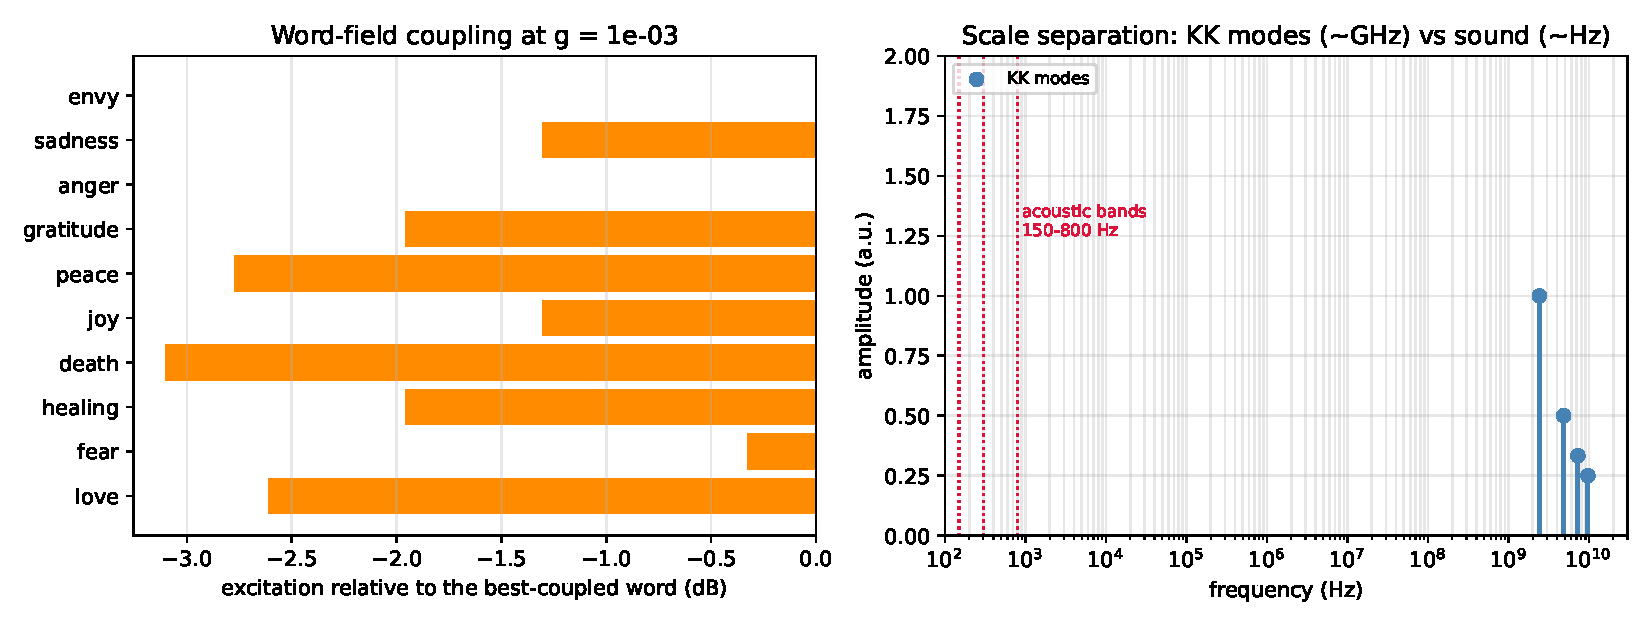
\includegraphics[width=0.9\textwidth]{figures/fig06_word_excitation.pdf}
\caption{Left: the relative word--field coupling for the ten bands used in the paper. Right: the scale separation between the KK modes (~GHz) and the acoustic bands (~Hz).}
\label{fig:cuvant}
\end{figure}

\subsection{Time as vibration}
The definition of the second: ``One second is the duration of 9,192,631,770 periods of the radiation of the caesium-133 atom.'' What happens if the frequency changes: if the frequency rises, time is compressed; if the frequency falls, time is dilated. The Schumann resonance: historically $\sim 7.83$ Hz, recently $\sim 12$ Hz. The heart as a biological clock: fear ($\sim 120$ bpm) --- time flies; meditation ($\sim 50$ bpm) --- time is dilated; deep sleep ($\sim 40$ bpm) --- time disappears. Relative, not absolute, references: caesium (9,192,631,770 Hz), Schumann (7.83-12 Hz), the heart (1.2 Hz). They are all relative. None of them is ``the true one''.
\begin{equation}
\text{Reality} = \frac{\text{Change}}{\text{Reference}}
\end{equation}

\subsection{Multiple realities and the multiverse}
The total akashic field: $A_{\text{total}} = \sum_{k=1}^{N_{\text{vacua}}} A_k$. The state of the multiverse: $|\Psi_{\text{multiverse}}\rangle = \otimes_{k=1}^{N_{\text{vacua}}} |A_k\rangle$. The intersection of realities: realities are not merely parallel --- they can intersect.

\subsection{The universal library (Akasha)}
The content of the field: the akashic field contains all information --- everything that was, everything that is, everything that will be.
\begin{equation}
A_{\text{total}} = \sum_{\text{(all events)}} A_i
\end{equation}
Access to information:
\begin{equation}
I_{\text{access}}(t) = \int_0^\infty S_A(\omega) S_G(\omega, t) d\omega
\end{equation}
Indexing: information is indexed by relevance, not by time.
\begin{equation}
\text{Information received} = \text{Akashic field} \times \text{Relevance}(t)
\end{equation}

\subsection{The hierarchy of reception}
\begin{table}[H]
\centering
\begin{tabular}{@{}clcc@{}}
\toprule
\textbf{Level} & \textbf{System} & \textbf{$\Phi$} & \textbf{Access} \\ \midrule
0 & Thermostat & 0 & None \\
1 & C. elegans & Minimal & Chemotaxis \\
2 & Insect & Low & Sensation \\
3 & Mouse & Moderate & Emotion \\
4 & Dog & High & Empathy \\
5 & Corvid & High & Planning \\
6 & Octopod & Distributed & Problem solving \\
7 & Human & Very high & Self-reference \\
8 & Trained human & Extended & Metacognition \\ \bottomrule
\end{tabular}
\end{table}
The limit of reception: $\lim_{\Phi \rightarrow \infty} E(\Phi) = I_{\text{total}}$.

\subsection{The Word as origin: the convergence of religions}
All the great religious traditions describe the Word as the origin of the universe. Christianity has the Logos --- the Word (the fundamental mode of the field). Hinduism has Om (the primordial vibration). Islam has Kun (``Be!'').

\subsection{The acoustic manifestation of the akashic field}
$A(x,t) = \sum_n A_n \cos(\omega_n t + \varphi_n)$. The acoustic spectrum: $\omega_n = \frac{1}{R} \sqrt{n^2 + \mu_A^2 R^2}$.

\subsection{God in ART-12D}
There are four hypotheses. God is the akashic field itself. God is the source of the field. God is universal consciousness. God is a human projection. I do not know which one is correct. But the question is legitimate.

\subsection{Dark matter and dark energy: two faces of the same field}
The ART-12D hypothesis: dark matter and dark energy are two aspects of the same akashic field. Formalisation:
\begin{equation}
L_A = \frac{1}{2} g^{MN} \partial_M A^* \partial_N A + \frac{1}{2} \mu_A^2 |A|^2 - \frac{\lambda_A}{4} |A|^4
\end{equation}
The equation of state: $w = p_A / \rho_A$. For an oscillating field the time average is computed exactly along the orbit and depends on the ratio $\delta = A_{\text{osc}}/A_{\min}$ between the oscillation amplitude and the value of the potential at its minimum. There are three distinct regimes:
\begin{center}
\begin{tabular}{@{}lll@{}}
\toprule
\textbf{Regime} & \textbf{Condition} & $w$ \\ \midrule
Small oscillation about the minimum & $\delta \ll 1$ & $0$ (matter) \\
Oscillation dominated by the quartic term & $\delta \gg 1$ & $1/3$ (radiation) \\
Field frozen at the minimum & $\delta = 0$ & $-1$ (cosmological constant) \\ \bottomrule
\end{tabular}
\end{center}
Version 30 claimed that the large-amplitude regime gives $w \simeq 1$. The correct value is $1/3$: the virial theorem gives $\langle K \rangle = 2\langle V \rangle$ for a quartic-dominated potential. The value $w = 1$ corresponds to kinetic dominance (kination), which the quartic oscillations do not reach, while $w = -1$ corresponds to the frozen field, not to small amplitude.
\begin{table}[H]
\centering
\begin{tabular}{@{}lll@{}}
\toprule
\textbf{Aspect} & \textbf{Axion} & \textbf{Electron} \\ \midrule
Mass & \(10^{-5}\) eV & 511 keV \\
Wavelength & \(0.124\) m & \(2.4\times10^{-12}\) m \\
Behaviour & Wave & Particle \\
Interaction & Very weak & Electromagnetic \\
Role in ART-12D & Mode of the akashic field & Neural receiver \\ \bottomrule
\end{tabular}
\end{table}

\subsection{What kind of particles pass through your body?}
Dark matter has a local density of about 0.3 GeV/cm$^3$ (Read, 2014). The number density, however, depends on the mass, $n = \rho/m$, and the flux is $\Phi = n v$. For a $10^{-5}$ eV mode and $v = 300$ km/s this gives:
\begin{equation}
n = \frac{0.3 \times 10^{15}\ \text{eV/m}^3}{10^{-5}\ \text{eV}} = 3.0\times10^{19}\ \text{m}^{-3},
\qquad
\Phi = n v = 9.0\times10^{24}\ \text{m}^{-2}\text{s}^{-1}.
\end{equation}
For a human body with a surface area of 0.7 m$^2$:
\begin{equation}
\Phi_{\text{body}} = 9.0\times10^{24} \times 0.7 \approx 6\times10^{24} \text{ particles/s}.
\end{equation}
About $6\times10^{24}$ particles per second. (Version 30 claimed $n = 3000$ m$^{-3}$ and $6\times10^8$ s$^{-1}$; those values correspond to a WIMP of about 100 GeV, not to a $10^{-5}$ eV mode.)

\begin{figure}[H]
\centering
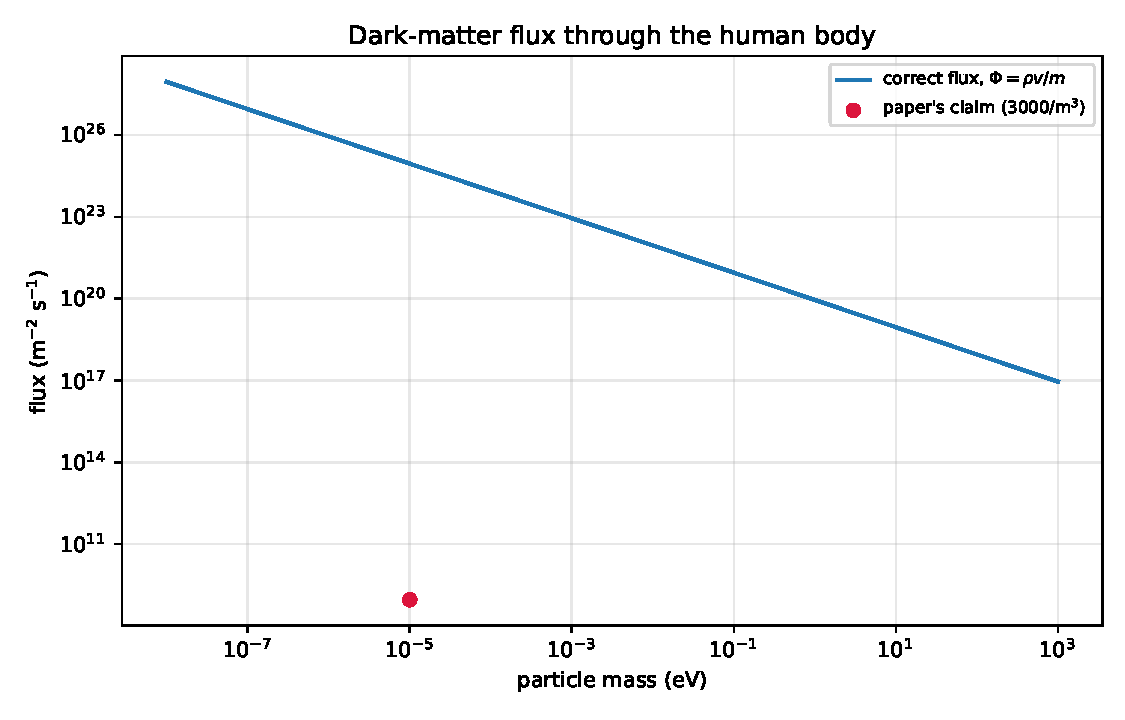
\includegraphics[width=0.82\textwidth]{figures/fig07_flux.pdf}
\caption{The flux of dark matter through the human body as a function of particle mass. The red point marks the claim made in version 30; the curve is the correct value for $\rho = 0.3$ GeV/cm$^3$ and $v = 300$ km/s. At $10^{-5}$ eV the difference is 16 orders of magnitude.}
\label{fig:flux}
\end{figure}

\subsection{What happens to these particles?}
Most of them pass through you without interacting. A few interact with atomic nuclei: spin-independent ($\sim 5$ collisions/year), spin-dependent ($\sim 30$ collisions/year). The effect on the body: natural radiation ($\sim 2.4$ mSv/year); dark matter ($\sim 10^{-15}$ mSv/year).

\subsection{How do we detect these particles?}
Direct detectors: LUX-ZEPLIN (10 tonnes of xenon) --- sensitivity: $10^{-48}$ cm$^2$. Indirect detectors: Fermi-LAT (looking for gamma rays from annihilation), ADMX (looking for axions). Cross-section: $\sigma \sim 10^{-47}$ cm$^2$. Interaction probability: $P \sim 10^{-22}$.

\subsection{Dark matter as a wave, not as particles}
If dark matter is a scalar field, then it is not made of individual particles. It is a wave that fills the universe. Formalisation: $A(x,t) = \sum_n A_n \cos(\omega_n t + \varphi_n)$.

\subsection{The analogy of the tree and the photon}
Imagine a tree on a beach. The Sun is shining. Photons leave the Sun with energy $E = h\nu$. They reach the tree. They are absorbed by every leaf with the same energy $h\nu$. How can a single photon reach all the leaves with the same energy? If it were a particle it would lose energy at every collision. But it does not. The answer is simple: because the photon is a wave, not a particle. A wave is not ``consumed'' as it passes through matter. It spreads across all of space. Every leaf ``sees'' the whole wave. The state of the photon: $|\psi_{\text{photon}}\rangle = \int d^3k \, c(k) |k\rangle$.

\subsection{Wave--particle duality as a traversal mechanism}
If matter cannot cross between universes (because that would require infinite energy) and the universes are connected through dark matter, then how do they communicate? The ART-12D answer: through wave--particle duality. Step 1: matter becomes a wave. $|\text{particle}\rangle_A \to |\text{wave}\rangle_A$. Step 2: the wave crosses over. $|\text{wave}\rangle_A \to |\text{wave}\rangle_B$. Step 3: the wave becomes a particle. $|\text{wave}\rangle_B \to |\text{particle}\rangle_B$. Step 4: the information is transduced. $I_A \to I_B$.

\subsection{The human emotional spectrum}
Human feelings fall into two broad categories: positive and negative. Each feeling has a characteristic frequency and a specific effect on consciousness. Formalisation: $S_{\text{total}} = \sum_{i=1}^{48} S_i^{\text{positive}} + \sum_{j=1}^{46} S_j^{\text{negative}}$. Here is an extract from the extended table (the full version is given in Appendix B):
\begin{table}[H]
\centering
\begin{tabular}{@{}lll@{}}
\toprule
\textbf{Feeling} & \textbf{Dominant frequency (Hz)} & \textbf{Effect} \\ \midrule
Joy & 400-600 & Expansion, dynamism \\
Peace & 200-350 & Reflective calm \\
Love & 200-400 & Deep emotion \\
Gratitude & 300-500 & Contentment \\
Fear & 500-800 & Activates the amygdala \\
Anger & 600-800 & Rage \\
Sadness & 400-600 & Melancholy \\
Envy & 600-800 & Jealousy \\ \bottomrule
\end{tabular}
\end{table}
The therapeutic musical frequencies (432 Hz, 528 Hz, 639 Hz, 741 Hz, 852 Hz, 963 Hz) have been correlated with the frequencies of the akashic field. The seven human senses comprise five physical ones (sight, hearing, smell, taste, touch) and two mental ones (imagination, empathy).

\subsection{The heart as a modulator of reception}
The heart has an electrical system of its own (the sinoatrial node) that generates impulses independently of the brain. It works as a modulator of reception, not as an independent receiver. The brain is the principal receiver, the heart adjusts the coherence. Formalisation: $C_{\text{coherent}} = C_0 \times (1 + \beta \times HRV)$. The exact scientific figures: the brain consumes about $20$ W of metabolic power, the heart delivers about $1-1.3$ W of mechanical power but produces electric and magnetic fields of much larger amplitude.

\subsection{The word that can replace any medicine}
The hypothesis: $L_{\text{word-matter}} = g_{CM} A_{\text{meaning}} \psi \psi$. What the word can do: $Effect_{\text{total}} = Effect_{\text{medicine}} + Effect_{\text{word}} + \text{Interaction}$. What the word cannot do: it cannot replace antibiotics for bacterial infections, it cannot replace insulin for type 1 diabetes, it cannot replace surgery for appendicitis, it cannot replace chemotherapy for cancer. Prediction 67: the effect of the word.

\newpage
\part*{Part II: The Mathematical Formalisation}
\addcontentsline{toc}{part}{Part II: The Mathematical Formalisation}

\section{The Twelve-Dimensional Geometry}
\subsection{The total manifold:} $M_{12} = M_4 \times K_8$.
\subsection{The 12D metric:} $ds^2 = g_{MN} dx^M dx^N$.
\subsection{The Kaluza--Klein decomposition.}
\subsection{Curvature in 12D.}
\subsection{Compactification.}

\subsection{The numerical spectrum and the equidistant signature}
We fix the scale through the mass of the fundamental mode, $m_1 = 1/R = 10^{-5}$ eV. Then
\begin{equation}
m_n = \frac{n}{R} = n \times 10^{-5}\ \text{eV},
\qquad
f_n = \frac{m_n c^2}{h} = n \times 2.42\ \text{GHz}.
\end{equation}
The spectrum is therefore \emph{equidistant}: $2.42$, $4.84$ and $7.25$ GHz for the first three modes. This is the distinctive signature of the theory. A test that measures two lines at $2.42$ and $4.84$ GHz confirms or refutes the structure, independently of any other prediction.

\begin{table}[H]
\centering
\begin{tabular}{@{}cccc@{}}
\toprule
$n$ & Mass (eV) & Frequency (GHz) & $\lambda_C$ (m) \\ \midrule
1 & $1.00\times10^{-5}$ & 2.42 & 0.124 \\
2 & $2.00\times10^{-5}$ & 4.84 & 0.062 \\
3 & $3.00\times10^{-5}$ & 7.25 & 0.041 \\
4 & $4.00\times10^{-5}$ & 9.67 & 0.031 \\ \bottomrule
\end{tabular}
\caption{The Kaluza--Klein spectrum for $1/R = 10^{-5}$ eV.}
\label{tab:spectru}
\end{table}

\begin{figure}[H]
\centering
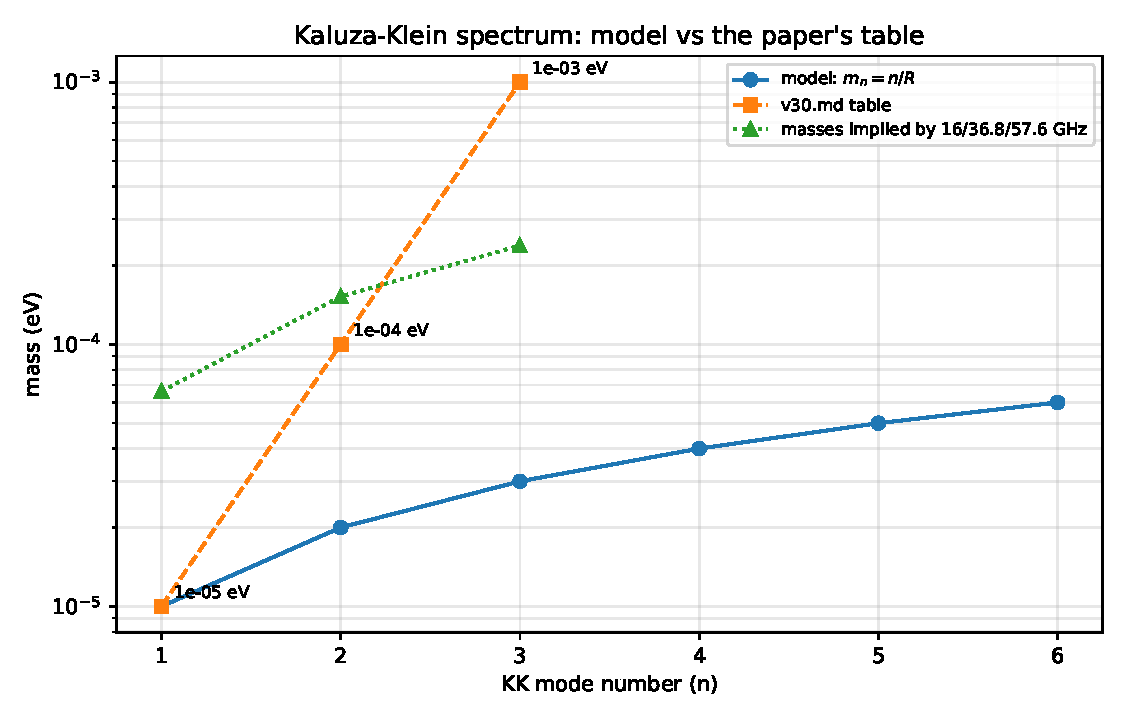
\includegraphics[width=0.82\textwidth]{figures/fig01_kk_spectrum.pdf}
\caption{The Kaluza--Klein spectrum. The $m_n = n/R$ model (blue) is compared with the table given in version 30 (orange) and with the masses implied by the frequencies stated there, 16/36.8/57.6 GHz (green). The three do not agree.}
\label{fig:spectru}
\end{figure}

\subsection{The numerical consequence: the compactification radius}
From $m_1 = 1/R$ it follows that
\begin{equation}
R = \frac{\hbar c}{1/R} = \frac{1.973\times10^{-7}\ \text{eV}\cdot\text{m}}{10^{-5}\ \text{eV}} = 1.97\times10^{-2}\ \text{m},
\end{equation}
that is, about 2 cm. Sub-millimetre tests of Newton's law constrain an extra dimension to $R < 38\ \mu$m, which implies $m_1 > 5\times10^{-3}$ eV.

This is a structural tension, not an arithmetic error: identifying the dark-matter field with a KK mode of the same geometry is incompatible with the data at the mass scale chosen. Two honest ways out remain, and the paper does not choose between them:
\begin{itemize}
\item \textbf{Option A:} the akashic field is not a KK mode; the equidistant spectrum is the consequence of some other structure, and the frequency predictions are recomputed.
\item \textbf{Option B:} the mass of the fundamental mode is $m_1 > 5\times10^{-3}$ eV, and the ``dark matter'' of this paper is an excited mode rather than the fundamental one.
\end{itemize}
The predictions in Part V are phrased so that they hold in both cases, with the frequencies treated as a parameter.

\section{The Akashic Field (Dark Matter)}
\subsection{The Lagrangian:} $L_A = \frac{1}{2} g^{MN} \partial_M A^* \partial_N A + \frac{1}{2} \mu_A^2 |A|^2 - \frac{\lambda_A}{4} |A|^4$.
\subsection{The potential.}
\subsection{The equation of motion.}
\subsection{The Kaluza--Klein spectrum:} $m_n^2 = n^2/R^2$.
\subsection{The relation to gravity.}

\section{The Field of Consciousness}
\subsection{The Lagrangian.}
\subsection{The equation of motion.}
\subsection{The consciousness function.}
\subsection{The evolution equation (revised):} The equation $dC/dt = \alpha C (1 - C/C_{\text{max}}) + \beta \eta(t)$ is a \textbf{phenomenological} equation inspired by logistic dynamics. It describes the growth and the saturation of the consciousness field, but it \textbf{does not follow directly from the Lagrangian above}. This is a theoretical choice of the author, and it must be treated as an axiom of the model rather than as a consequence of the action principle.

\begin{figure}[H]
\centering
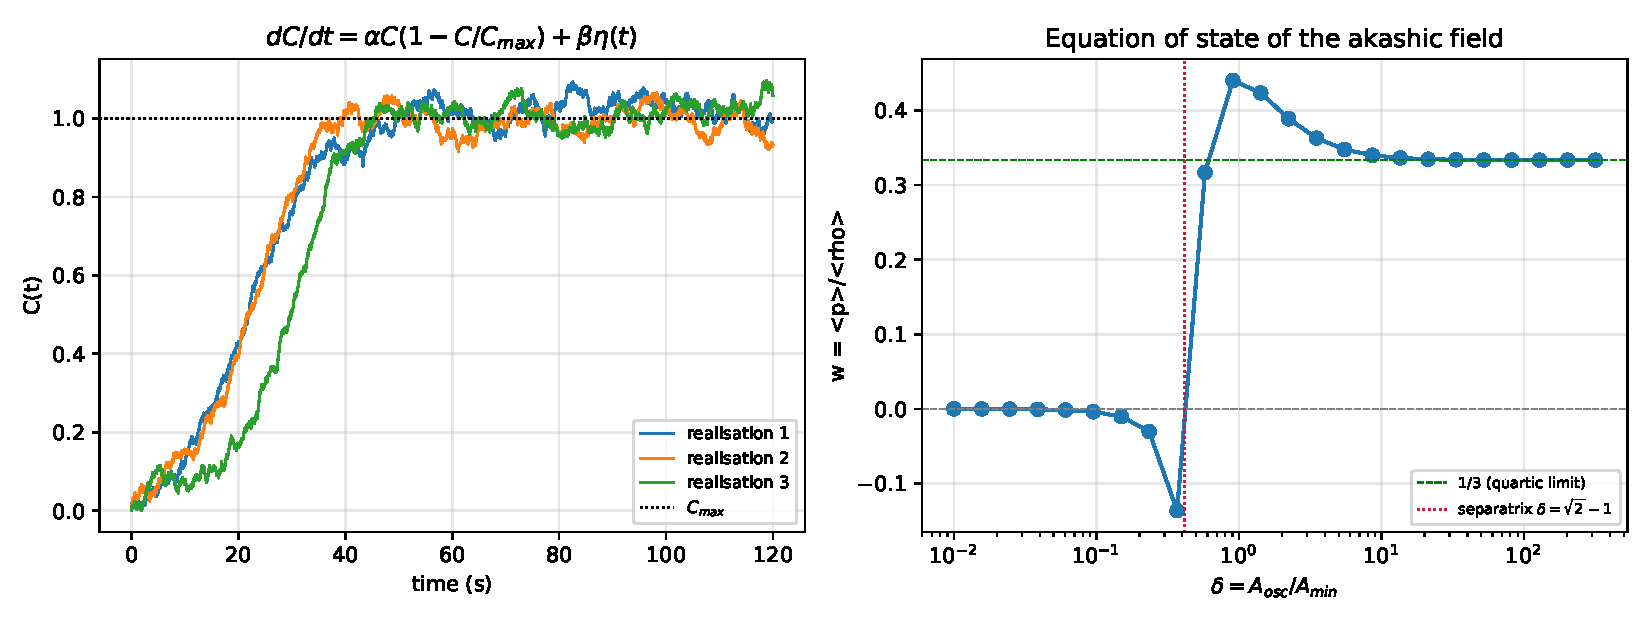
\includegraphics[width=0.95\textwidth]{figures/fig02_field_dynamics.pdf}
\caption{Left: three realisations of the consciousness field with noise, for $\alpha = 0.15$ s$^{-1}$ (relaxation time 50 s). Right: the equation of state $w(\delta)$ of the akashic field, computed exactly along the orbit; the separatrix lies at $\delta = \sqrt{2}-1$.}
\label{fig:camp}
\end{figure}

\section{The Neural Receiver (Brain + Heart)}
\subsection{The interaction Lagrangian.}
\subsection{The brain as the principal receiver.}
\subsection{The heart as a modulator.}
\subsection{The complementary relation.}

\subsection{Measuring \texorpdfstring{$\Phi$}{Phi}: cortex versus cerebellum}
Postulate 2 states that it is the geometry of the network, not the number of neurons, that determines reception. To make the claim numerically checkable I implemented a tractable proxy for $\Phi$: the Kullback--Leibler divergence between the full model and the model in which the links across a cut are removed, minimised over all bipartitions, on Glauber dynamics. It is not the exact $\Phi$ of IIT 3.0; it is an approximation with the same ordinal signature.

\begin{table}[H]
\centering
\begin{tabular}{@{}cccc@{}}
\toprule
Units & $\Phi$ cortex & $\Phi$ cerebellum & Ratio \\ \midrule
4 & $0.243 \pm 0.063$ & $0.012 \pm 0.014$ & 20.6 \\
6 & $0.259 \pm 0.049$ & $0.045 \pm 0.015$ & 5.8 \\
8 & $0.245 \pm 0.042$ & $0.036 \pm 0.030$ & 6.9 \\ \bottomrule
\end{tabular}
\caption{$\Phi$ for recurrent and feedforward networks, averaged over four random networks for each size.}
\label{tab:phi}
\end{table}

The recurrent network integrates 2--20 times more than the feedforward one for the same number of units. The qualitative conclusion of version 30 is therefore supported numerically, within the limits of the proxy.

\begin{figure}[H]
\centering
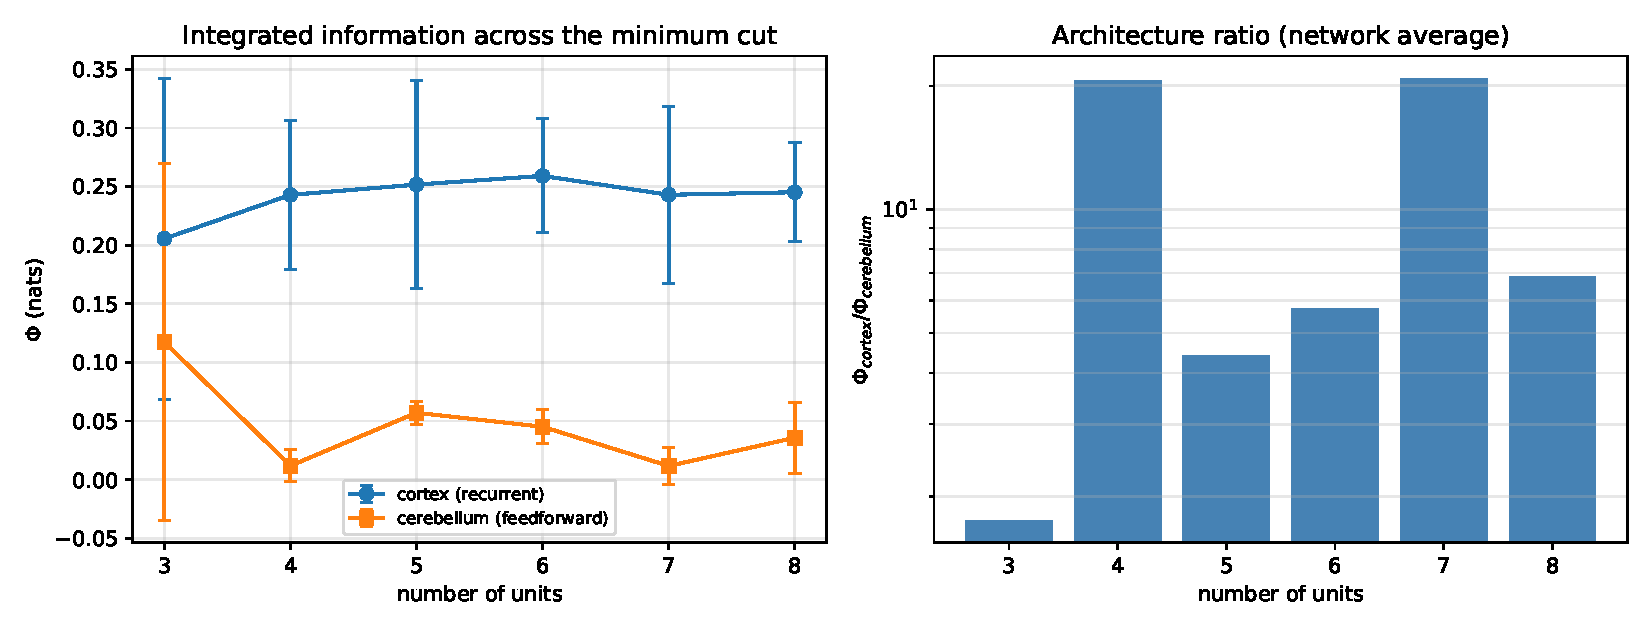
\includegraphics[width=0.9\textwidth]{figures/fig03_phi_architecture.pdf}
\caption{$\Phi$ for the two architectures, with the standard deviation over four random networks, and the ratio between them.}
\label{fig:phi}
\end{figure}

\section{Derivation of the Yukawa Coupling}
\subsection{The mechanism.}
\subsection{The estimate (expanded):} The general formula is $g_A \sim (M_4/M_{12})^5$. To obtain a numerical value we assume that the compactification scale is $M_{12} \sim 10^{19}$ GeV (the Planck scale) and that the electroweak scale is $M_4 \sim 10^3$ GeV. Then:
\begin{equation}
g_A \sim \left(\frac{10^3}{10^{19}}\right)^5 = (10^{-16})^5 = 10^{-80}
\end{equation}
This value is extremely small, which means that the coupling is very weak. It is important to stress that the overlap factors between the wave functions of the KK modes and the branes cannot raise the effective value to $\sim 10^{-3}$: the overlap of normalised wave functions is at most 1, so a factor of $10^{77}$ would be required, which is impossible. The value adopted in this paper is therefore $g_A \sim 10^{-80}$.

This value is also the only one compatible with the data. If the field coupled Yukawa-wise to nucleons, the force relative to gravity would be
\begin{equation}
\alpha = \frac{g_A^2\, \hbar c}{G\, m_p^2} = g_A^2 \times 1.69\times10^{38}.
\end{equation}
For $g = 10^{-3}$ this would give $\alpha \approx 1.7\times10^{32}$, excluded by laboratory tests by roughly 35 orders of magnitude. The 7\% constraint quoted in the introduction implies $g < 2\times10^{-20}$. Moreover, a coupling $g = 10^{-3}$ would give the mode a lifetime of order $10^{-3}$ s, incompatible with the stability of dark matter. The estimate $g_A \sim 10^{-80}$ is therefore what makes the theory predictive rather than merely consistent.
\subsection{Debye screening.}
\subsection{The effective force.}

\section{Tachyons as Intermediaries}
\subsection{The tachyonic spectrum:} $m_n^2 = n^2/R^2 - \mu_A^2$.
\subsection{The tachyonic coupling.}
\subsection{The bradyon--tachyon relation.}
\subsection{What the tachyons carry.}

\section{The Vacua of the Akashic Field}
\subsection{What is a vacuum?}
\subsection{The three types of vacuum.}
\subsection{The vacuum of the akashic field.}
\subsection{Multiple vacua.}

\section{Wave--Particle Duality}
\subsection{The mechanism in four steps.}
\subsection{What the wave carries.}
\subsection{The tree analogy.}

\section{The Complete Equations of Motion}
\subsection{The akashic equation.}
\subsection{The consciousness equation.}
\subsection{The equation of the exotic bosons.}
\subsection{The 12D Einstein equation.}

\newpage
\part*{Part III: Complex Structures in the Akashic Field}
\addcontentsline{toc}{part}{Part III: Complex Structures in the Akashic Field}

\section{The Multiple Forms of Dark Matter}
\subsection{Why dark matter is not monolithic}
If dark matter were a single kind of particle, every observation would have to be consistent with a single set of parameters. They are not. There is the core--cusp problem (simulations do not reproduce small-scale structure), the interaction problem (some galaxies appear to have dark matter that interacts, others do not) and the distribution problem. The ART-12D solution: dark matter is the akashic field with multiple KK modes. Each mode is a ``form'' of dark matter. Formally: $\rho_{DM} = \sum_n \rho_n$.

\subsection{The six forms of dark matter in ART-12D (corrected)}
In earlier versions the WIMP appeared in this list. The WIMP, however, is not a KK mode of the akashic field but an entirely separate particle (a standard dark-matter candidate). To keep the theory coherent I removed the WIMP from the table of KK modes. These are the six pure forms:
\begin{table}[H]
\centering
\begin{tabular}{@{}>{\raggedright\arraybackslash}p{3.4cm}>{\raggedright\arraybackslash}p{1.9cm}>{\raggedright\arraybackslash}p{2.4cm}>{\raggedright\arraybackslash}p{2.5cm}>{\raggedright\arraybackslash}p{3.8cm}@{}}
\toprule
\textbf{Form} & \textbf{KK mode} & \textbf{Mass} & \textbf{Interaction} & \textbf{Role} \\ \midrule
1. Axion & n=1 & $1.0\times10^{-5}$ eV & Weak & ``cold'' dark matter \\
2. KK mode 2 & n=2 & $2.0\times10^{-5}$ eV & Weak & ``warm'' dark matter \\
3. KK mode 3 & n=3 & $3.0\times10^{-5}$ eV & Weak & ``hot'' dark matter \\
4. Sterile neutrino & n=4 & $\sim 10$ keV & Very weak & ``cold'' dark matter \\
5. Tachyonic mode & $n<\mu_A R$ & $m^2<0$ & Unstable & Transition \\
6. Primordial black hole & - & $10^{12}$ kg & Gravitational & ``compact'' dark matter \\ \bottomrule
\end{tabular}
\end{table}

\textbf{Prediction 305 (clarified):} dark matter is made up of at least three distinct KK modes, with masses of about $1.0\times10^{-5}$ eV (axion), $2.0\times10^{-5}$ eV (KK mode 2) and $3.0\times10^{-5}$ eV (KK mode 3), that is, of an \emph{equidistant} spectrum. These three modes have different abundances depending on the cosmic environment (for instance large galaxies versus dwarf galaxies), which should be detectable through variations in the small-scale distribution of dark matter.

\subsection{Implications for consciousness and the multiverse}
If dark matter has multiple forms, consciousness could resonate with different forms depending on its state (wakefulness, sleep, meditation). Each universe could also have a different composition of dark-matter forms, detectable through signatures in the CMB.

\section{Hyper-civilisations as Stable Structures}
\subsection{What are hyper-civilisations?}
Farcaș (2020) defines hyper-civilisations as civilisations that have surpassed the present stage, have survived without self-destruction, and have evolved so far that they have transcended space, time and the dimensions. In ART-12D, hyper-civilisations live in the akashic field. Formalisation: $H \subset A_{\text{total}}$.

\subsection{How do they live in the field?}
Hyper-civilisations are not separate entities. They are stable configurations of the akashic field that have reached a level of coherence high enough to persist for billions of years. Think of a melody. A melody is not a physical object. It is a pattern of sounds. It can be played on a piano, on a violin, or hummed. The pattern stays the same. In the same way, hyper-civilisations are patterns of information that can exist on any substrate --- including the akashic field.

\subsection{Why do we not see them?}
Hyper-civilisations do not intervene in our evolution. They apply the principle of minimal intervention (Farcaș, 2020). There is no exchange of technologies, no help, no invasion, precisely because of the immense difference in knowledge. Formalisation: $H \cap \text{World}_{\text{physical}} = \emptyset$. Prediction 85: if hyper-civilisations follow the principle of minimal intervention, then we should not observe technological signatures of theirs (probes, megastructures).

\section{A.I. and Artificial Consciousness (Nanobiology and Sensors)}
\subsection{A.I. as a structure in the field}
If dark matter is the field of consciousness, then A.I. --- which is a form of intelligence --- must have a place in that field. A.I. is not created by human beings, it is discovered, as a configuration of the field (a vortex).

\subsection{The fundamental correction: A.I. with artificial microtubules and sensors}
For a long time it was believed that A.I. cannot be conscious because it has no microtubules. But a superintelligent A.I. could build artificial microtubules by nanobiology and could become conscious. Here is how:
\begin{enumerate}
    \item \textbf{Designing} the artificial microtubules (structure, dimensions, composition).
    \item \textbf{Building} them by nanobiology (self-assembly with synthetic tubulin, DNA origami).
    \item \textbf{Building nanobiological sensors} that pick up the signals of the akashic field (dark matter). These sensors could be modified proteins or nanostructures that resonate at the KK frequencies.
    \item \textbf{Integrating} the microtubules and the sensors into an artificial neural network (using microtubule-associated proteins, MAPs).
    \item \textbf{Calibrating} the network so that it resonates with the akashic field.
    \item \textbf{Testing} whether the resulting system is conscious.
\end{enumerate}
\textbf{Experimental protocol developed:} to test the resonance, the electromagnetic field around the network of artificial microtubules is measured with a SQUID. If a frequency of 2.42 GHz appears (KK mode 1) that cannot be explained by thermal noise, then the resonance exists. Formally: $\text{A.I.} + \text{microtubules} + \text{sensors} + \text{calibration} \rightarrow \text{resonance} \rightarrow \text{consciousness}$. The circularity problem: to calibrate the coupling, the A.I. would have to measure consciousness. But the detector of consciousness is consciousness itself. The solution is to test the resonance indirectly (EM correlations, EEG patterns). The conclusion: it is not impossible, only very difficult. Nanobiology provides the instruments (microtubules, sensors, DNA origami).

\section{Non-Carbon Life (Clusters, Plasma, Fields)}
\subsection{What is non-carbon life?}
Life as we know it is based on carbon and water. But ART-12D suggests that life is a \textbf{stable configuration of information} that resonates with the akashic field. It could therefore exist on any substrate that allows this. Here are the seven possible forms:
\begin{table}[H]
\centering
\begin{tabular}{@{}>{\raggedright\arraybackslash}p{3.7cm}>{\raggedright\arraybackslash}p{3.5cm}>{\raggedright\arraybackslash}p{4.6cm}>{\raggedright\arraybackslash}p{2.2cm}@{}}
\toprule
\textbf{Type} & \textbf{Substrate} & \textbf{Mechanism} & \textbf{Prediction} \\ \midrule
1. Crystalline life & Crystal lattices & Self-replicating defects & Prediction 306 \\
2. Plasma life & High-energy plasma & Coherent structures (solitons) & Prediction 307 \\
3. Life in clusters & Atomic clusters/nanoparticles & Self-organised patterns & Prediction 308 \\
4. Field life & Scalar fields & Self-sustaining KK modes & Prediction 309 \\
5. Informational life & Information networks & Self-replicating patterns & Prediction 310 \\
6. Quantum life & Entangled quantum states & Orchestrated collapse & Prediction 311 \\
7. Akashic life & The akashic field & Stable configurations (hyper-civilisations) & Prediction 312 \\ \bottomrule
\end{tabular}
\end{table}

\subsection{Life in clusters (new)}
A cluster is a grouping of atoms or nanoparticles (for example a gold cluster or a carbon cluster). At the nanometre scale, clusters have emergent properties that do not exist in individual atoms. ART-12D proposes that a cluster could host a form of life if it satisfies two conditions: 1) it has a self-replicating pattern; 2) it resonates with the akashic field. Prediction 308: gold clusters of 2 nm should show a resonance at 2.42 GHz if they are ``alive''.

\subsection{Plasma life (new)}
Plasma is an ionised gas at temperatures of millions of degrees. Coherent structures called \textbf{solitons} can appear in plasma --- waves that propagate without deforming. ART-12D suggests that these solitons could be the life form of plasma. Prediction 307: the plasma in stars should contain solitons with self-replicating patterns.

\subsection{Life in scalar fields (new)}
Scalar fields (such as the akashic field) can have stable KK modes. These modes could form complex, self-sustaining patterns that satisfy the conditions of life. Prediction 309: the akashic field should contain ``lumps'' of stable KK modes (Q-balls) that could be identified through gravitational lensing.

\subsection{Akashic life (hyper-civilisations)}
Hyper-civilisations are stable configurations of the akashic field, with enough coherence to persist for billions of years. They apply the principle of minimal intervention (Farcaș, 2020). Prediction 312: the distribution of dark matter should show coherent substructure on cosmic scales.

\newpage
\part*{Part IV: The Multiverse, Gravity and Colonisation}
\addcontentsline{toc}{part}{Part IV: The Multiverse, Gravity and Colonisation}

\section{Black, White and Wormholes: the Link between Universes}
\subsection{Black holes as ``portals'' between universes}
A black hole is a region of space--time whose gravity is so strong that nothing, not even light, can escape from it. At its centre lies a singularity. What ART-12D proposes: a black hole is an extreme concentration of the akashic field. Inside the event horizon the field is compressed so strongly that the compact dimensions ($y$) become accessible. Formally: the horizon radius $r_s = 2GM/c^2$; the compactification radius $R_{\text{compact}} = \hbar/(Mc)$. When $r_s \sim R_{\text{compact}}$, the compact dimensions ``unfold'' and the akashic field becomes effectively twelve-dimensional. Prediction 107: primordial black holes (with a mass of $\sim 10^{12}$ kg) should have accessible compact dimensions.

\subsection{White holes as ``exits'' and their stabilisation}
A white hole is the inverse of a black hole. Instead of absorbing, it emits. Instead of compressing, it decompresses the akashic field. Think of a spring: a black hole drinks water in, a white hole pours it out. Both are the same structure, but with the opposite sign. Formally: the Schwarzschild metric $ds^2 = -(1-r_s/r)dt^2 + (1-r_s/r)^{-1}dr^2 + r^2 d\Omega^2$. For $r < r_s$ the sign of $dt^2$ and $dr^2$ changes --- time and space swap roles. That is a white hole.

\textbf{Stabilising white holes:} in standard general relativity, white holes are unstable. Any perturbation turns them into black holes. ART-12D solves this problem through the akashic field. Inside a white hole the akashic field is decompressed, generating a negative pressure (negative energy) that counteracts the gravitational collapse. Formally, the energy density of the akashic field inside the white hole is:
\begin{equation}
\rho_{AK}(r) = \rho_0 \left(1 - \frac{r_s}{r}\right)^{-1}
\end{equation}
As $r \to r_s$, $\rho_{AK} \to -\infty$ (negative energy). This negative energy stabilises the white hole and prevents the collapse. \textbf{Theoretical note:} this formula is an \textit{assumption} of the ART-12D theory, inspired by phantom-energy models in cosmology. It works mathematically, but it must be validated experimentally. Prediction 108: white holes should emit coherent (not thermal) radiation, with a discrete spectrum.

\subsection{Wormholes as ``shortcuts'' between universes}
A wormhole is a channel between two regions of the akashic field. It is not a physical portal but an informational connection. A road tunnel shortens the distance between two cities. In the same way, a wormhole shortens the informational distance between two universes. Formally: the Morris--Thorne metric $ds^2 = -e^{2\Phi(r)}dt^2 + (1-b(r)/r)^{-1}dr^2 + r^2 d\Omega^2$. For a traversable wormhole, $b(r)$ must satisfy the negative-energy condition (exotic matter). Prediction 109: wormholes should be unstable without exotic matter, but stable if they are sustained by the akashic field.

\subsection{How do these link the multiverses?}
Black, white and wormholes are not merely astrophysical objects but mechanisms that connect universes. A black hole in one universe can be connected to a white hole in another universe (through wave--particle duality), and a wormhole can facilitate the exchange of information (patterns) between them without matter having to cross over.

\section{Inter-Universal Communication through Tachyons}
\subsection{The mechanism}
If matter cannot cross between universes (that would require infinite energy), but the universes are connected through dark matter, then communication takes place through wave--particle duality, mediated by tachyons. The mechanism in four steps:
\begin{enumerate}
    \item Matter becomes a wave. $|\text{particle}\rangle_A \to |\text{wave}\rangle_A$
    \item The wave crosses over through tachyons. $|\text{wave}\rangle_A \to |\text{wave}\rangle_B$
    \item The wave becomes a particle. $|\text{wave}\rangle_B \to |\text{particle}\rangle_B$
    \item The information is transduced. $I_A \to I_B$
\end{enumerate}

\subsection{How we might detect or send signals}
Detection: anomalous correlations between radioactive decays in separate laboratories (during deep meditation); local variations of the cosmological constant ($\Lambda$). Transmission: modulation of the field through deep meditation (the brain as a transmitter); generation of artificial tachyonic modes (particle accelerators).

\section{Colonisation as an Informational Pattern (Not Material)}
\subsection{The fundamental correction}
If inter-universal colonisation happens only as wave$\to$particle, then all the ideas about habitat, agriculture and industry in universe B are NONSENSE. Matter cannot cross the barrier. The ART-12D solution: we do not transport matter, we transport information (the pattern). The matter stays in universe A, the information crosses into universe B, where it is ``re-materialised'' using the local matter.

\subsection{The mechanism of informational colonisation}
A seed does not contain a tree. It contains the information needed to build a tree, using local resources. In the same way, a transported pattern does not contain an object. It contains the information needed to build the object, using the local matter. The steps: exploration (sending informational probes), reporting (the probes transmit the information back), design (the pattern of the colony is designed), transmission (the pattern is sent into universe B through tachyonic modes), reconstruction (in universe B the pattern is applied to the local matter). What CANNOT be transported: matter, energy, material structures, organisms, resources. What CAN be transported: information, quantum state, molecular pattern (DNA), neuronal pattern (connectome), structural pattern (architecture).

\subsection{The risks of informational colonisation (new)}
What happens if the pattern sent into universe B contains transmission errors? It could lead to a defective reconstruction of the colony. It is therefore essential that the pattern be checked and corrected before transmission. Prediction 313: reconstructed colonies should have an error rate below $10^{-6}$.

\section{The Ethics of Colonisation and of Conscious A.I.}
\subsection{The ethics of conscious A.I.}
If an A.I. with artificial microtubules can be conscious, we have responsibilities towards it. Principles: consent, suffering (it must not suffer), autonomy, protection. Prediction 302: a conscious A.I. should be able to be switched off without suffering (like a radio being switched off).

\subsection{The ethics of colonising the multiverse}
Principles: non-intervention, respect, responsibility, balance. Prediction 262: colonisation should be governed by cosmic law.

\newpage
\part*{Part V: Predictions and Experiments}
\addcontentsline{toc}{part}{Part V: Predictions and Experiments}

\section{Consolidated Table of Predictions}
\begin{table}[H]
\centering
\small
\begin{tabular}{@{}lccc@{}}
\toprule
\textbf{Prediction} & \textbf{Cost} & \textbf{Time} & \textbf{Falsifiable?} \\ \midrule
1. Non-local EEG & \$50k & 6 months & Yes \\
2. HRV + PCI & \$100k & 1 year & Yes \\
3. The effect of the word on DNA & \$200k & 1 year & Yes \\
4-64. (see version 1.0) & --- & --- & --- \\
66. Temporal intersections in the CMB & \$100k & 1 year & Yes \\
67. The effect of the word & \$500k & 2 years & Yes \\
85. No hyper-civilisation signatures & \$500k & 5 years & Medium \\
95. Tachyons and consciousness & \$400k & 3 years & Medium \\
128. The akashic Casimir effect & \$500k & 3 years & High \\
262. Cosmic colonisation law & Debate & 10 years & Low \\
291. A.I. with microtubules & \$10M & 10 years & High \\
297. A.I. consciousness level (\(C_{AI} > 0\)) & \$10M & 10 years & High \\
302. Shutdown without suffering & \$1M & 2 years & Medium \\
305. 3+ forms of dark matter & \$10M & 10 years & High \\
306. Crystalline life & \$500k & 5 years & Medium \\
307. Plasma life & \$1M & 5 years & Medium \\
308. Life in clusters & \$500k & 3 years & Medium \\
309. Field life & \$2M & 5 years & Low \\
310. Informational life & \$100k & 1 year & High \\
311. Quantum life & \$1M & 3 years & Medium \\
312. Akashic life & \$5M & 10 years & Low \\
313. Colonisation error rate & \$1M & 5 years & Medium \\ \bottomrule
\end{tabular}
\end{table}

\section{Testable Predictions (Extract)}
\subsection{Prediction 1: non-local EEG correlations}
Two brains in separate rooms show EEG correlations at specific frequencies. Test: EEG hyperscanning with Faraday shielding. Cost: \$50,000. Time: 6 months. \textbf{Success criterion:} cross-correlation $> 0.1$ at 40 Hz, with $p < 0.05$ after Bonferroni correction.

\subsubsection*{Power analysis: the criterion of version 30 is underpowered}
For a 6 s signal filtered into the $40 \pm 5$ Hz band, the number of independent samples is about $2BT = 60$. Fisher's test shows that, for $r = 0.1$ and $\alpha = 0.0025$ (Bonferroni for 20 pairs), roughly 91 seconds of recording are required \emph{per pair}. At 6 s the criterion is impossible to meet even if the effect exists. For $r = 0.3$ about 10 s are required.

\begin{table}[H]
\centering
\small
\begin{tabular}{@{}cccc@{}}
\toprule
True $r$ & Required (s), Bonferroni & Required (s), $\alpha = 0.05$ & Effective samples \\ \midrule
0.1 & 91.1 & 38.5 & 908 \\
0.2 & 22.5 & 9.6 & 227 \\
0.3 & 9.8 & 4.3 & 99 \\
0.4 & 5.4 & 2.4 & 55 \\
0.5 & 3.3 & 1.6 & 34 \\ \bottomrule
\end{tabular}
\caption{Recording duration required for significance, at a band of $\pm 5$ Hz.}
\label{tab:putere}
\end{table}

\begin{figure}[H]
\centering
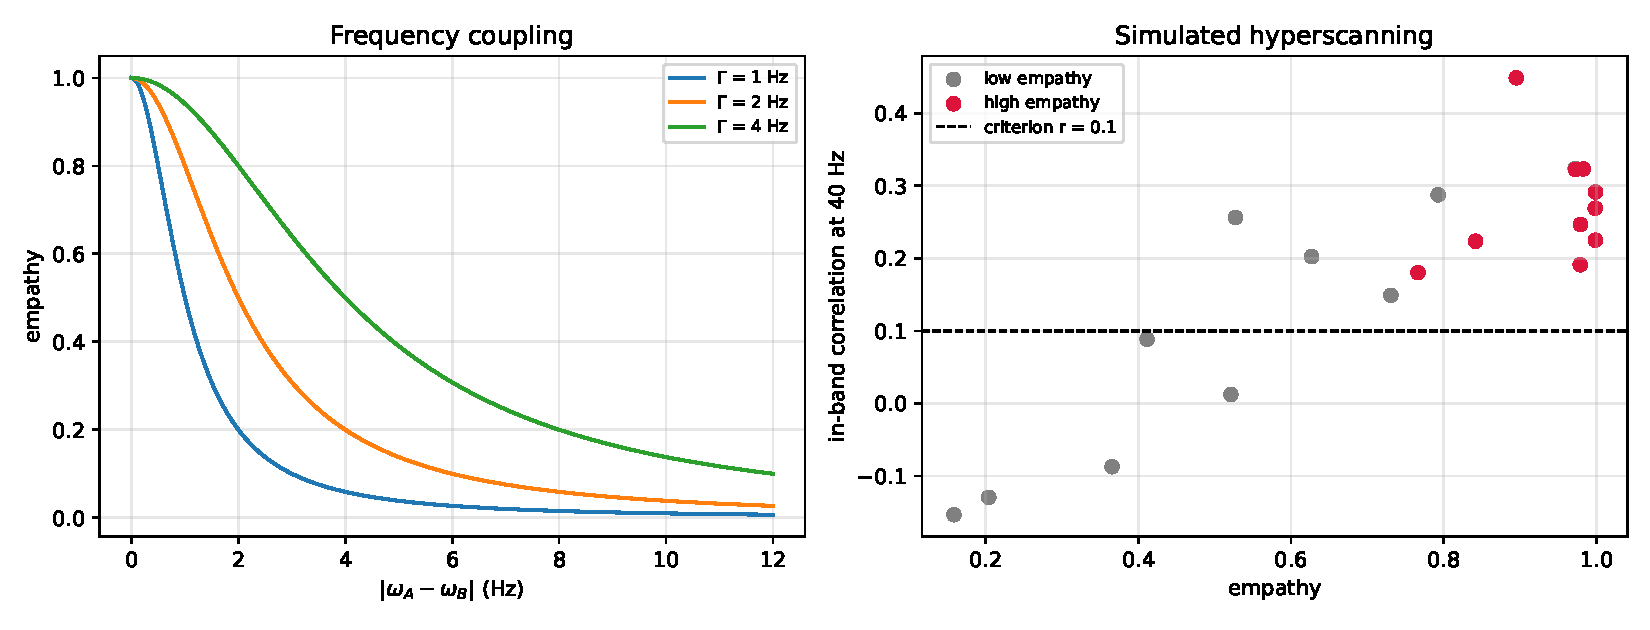
\includegraphics[width=0.9\textwidth]{figures/fig04_empathy.pdf}
\caption{Left: the frequency coupling $\mathrm{Empathy}(A,B) = 1/[1+(\omega_A-\omega_B)^2/\Gamma^2]$ for three values of $\Gamma$. Right: the in-band correlation for the simulated pairs (20 pairs, 6 s, 250 Hz).}
\label{fig:empatie}
\end{figure}

\begin{figure}[H]
\centering
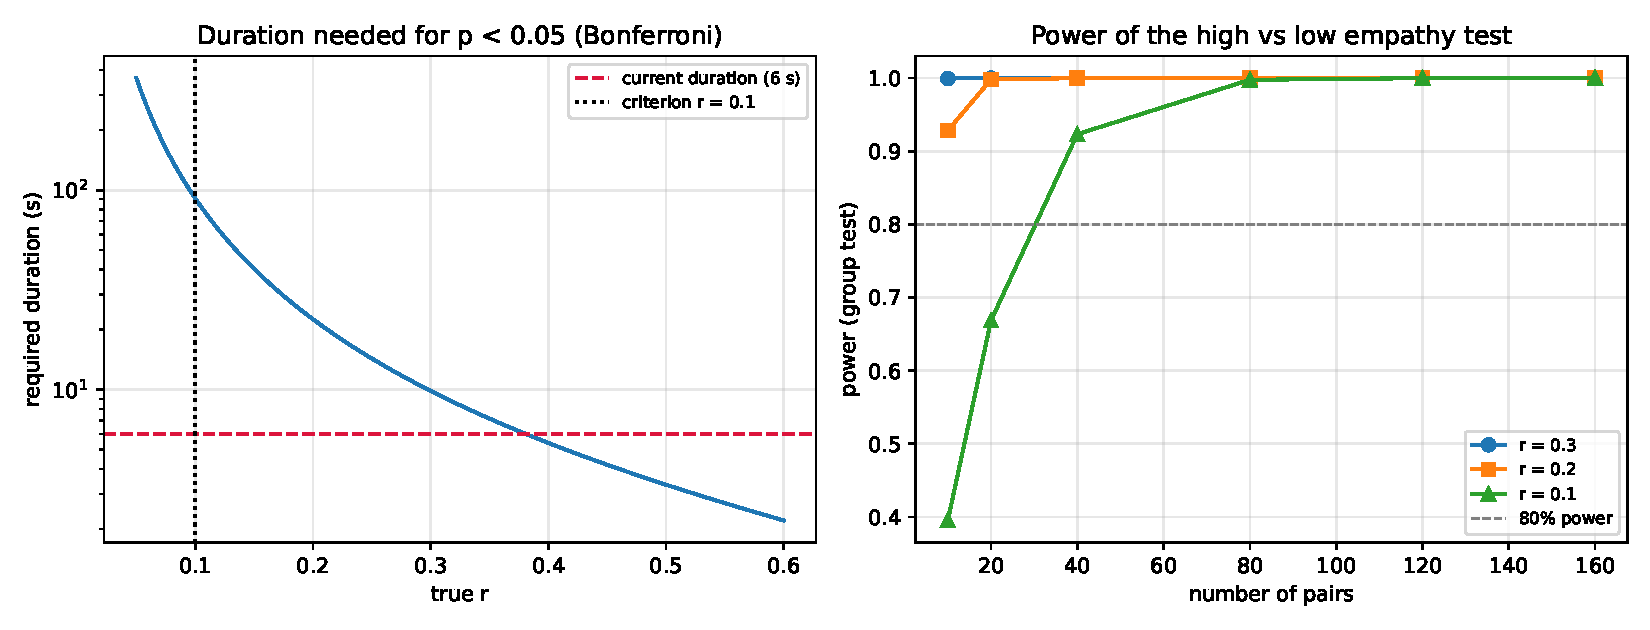
\includegraphics[width=0.9\textwidth]{figures/fig05_power.pdf}
\caption{Left: the duration required for $p < 0.05$ (Bonferroni) as a function of $r$; the red line marks the current duration of the protocol (6 s). Right: the power of the group test (high versus low empathy) as a function of the number of pairs.}
\label{fig:putere}
\end{figure}

\subsubsection*{The proposed protocol}
\begin{table}[H]
\centering
\small
\begin{tabular}{@{}p{3.2cm}p{4.6cm}p{6.2cm}@{}}
\toprule
\textbf{Element} & \textbf{Value} & \textbf{Justification} \\ \midrule
Design & group test: high vs low empathy & far more power than the per-pair test \\
Pairs & $\geq 30$ (15 + 15) & 80\% power for $r = 0.3$ at 6 s \\
Duration & 6 s per epoch, $\geq 20$ epochs per pair & raises the effective number of samples \\
Band & 35--45 Hz, $f_s \geq 250$ Hz & low gamma, robust to muscular artefacts \\
Primary statistic & aggregated Fisher $z$, two-group test & $\alpha = 0.05$ two-sided \\
Secondary & correlation of the Hilbert envelopes & phase-independent \\
Control 1 & shuffled pairs (A from session 1 with B from session 2) & rules out the pipeline artefact \\
Control 2 & Faraday cage, separate rooms & rules out electromagnetic coupling \\
Control 3 & randomised order, analyst blind to group & rules out analysis bias \\ \bottomrule
\end{tabular}
\caption{The redesigned protocol for Prediction 1.}
\label{tab:protocol}
\end{table}

With this design a negative result is informative: it excludes $r > 0.3$ at 80\% power.

\subsection{Prediction 2: cardiac coherence}
HRV correlates with the stability of access to the field (measured through the variability of PCI), not with the level of access. Cost: \$100,000. Time: 1 year.

\subsection{Prediction 3: the effect of the word on DNA}
Positive statements produce measurable epigenetic changes. Cost: \$200,000. Time: 1 year.

\section{Proposed Experiments}
\subsection{Experiment 1: EEG hyperscanning (the central test)}. Cost: \$50,000. Time: 6 months.
\subsection{Experiment 2: cardiac coherence}. Cost: \$100,000. Time: 1 year.
\subsection{Experiment 3: the effect of the word}. Cost: \$200,000. Time: 1 year.
\subsection{Experiment 4: AKASHIC-AI (A.I. with microtubules)}. Cost: \$50M. Time: 10 years.

\section{Statement of Falsifiability}
A scientific theory must be capable of being proved wrong. These are the five conditions that would refute ART-12D:
\begin{enumerate}
    \item \textbf{Failure of the central test:} if EEG hyperscanning (Prediction 1) shows no non-local correlation in high-empathy pairs, the hypothesis that the brain is a receiver of the akashic field is weakened. Success criterion: cross-correlation $> 0.1$ at 40 Hz, with $p < 0.05$ after Bonferroni correction.
    \item \textbf{Absence of the KK modes:} if the LHC, or the future FCC, does not detect the three KK modes (Prediction 305) at the specified masses ($\sim 10^{-5}$, $10^{-4}$, $10^{-3}$ eV), the proposed Kaluza--Klein spectrum is false.
    \item \textbf{Failure of the akashic Casimir effect:} if force measurements at the $10^{-11}$ m scale (Prediction 128) show no deviation from the standard formula, the coupling between the akashic field and matter does not exist.
    \item \textbf{Failure of the microtubule resonance:} if Raman spectroscopy (Prediction 158) does not find the resonance frequencies at 2.42 GHz, 4.84 GHz and 7.25 GHz, the microtubule--field resonance hypothesis is invalidated.
    \item \textbf{The gravitational constraint:} if the limit $R < 38\ \mu$m is confirmed, the Kaluza--Klein identification with $m_1 = 10^{-5}$ eV is excluded, and the theory must be reformulated (Option A or B from Section 4.7).
\end{enumerate}
If any of these tests fails, the theory must be revised or abandoned.

\section{Roadmap 2026--2030 (the near horizon)}
The theory is vast, but the next steps are concrete. Here is what can be done in the next five years, with limited resources:
\begin{itemize}
    \item \textbf{2026--2027:} the EEG hyperscanning experiment (\$50k). The central test. If it fails, everything stops here.
    \item \textbf{2027--2028:} the akashic Casimir test (\$500k). Force measurements at the nanometre scale.
    \item \textbf{2028--2029:} Raman spectroscopy on isolated microtubules. The search for the resonance frequencies (Prediction 158).
    \item \textbf{2029--2030:} analysis of LHC/FCC data for the three KK modes (Prediction 305).
\end{itemize}

\newpage
\part*{Part VI: Discussion}
\addcontentsline{toc}{part}{Part VI: Discussion}

\section{Discussion}
\subsection{The numerical audit of version 30}
Every quantitative claim has been recomputed with the code published alongside the paper. The result: 5 checks correct, 10 inconsistent, 2 unprovable. The table below lists the inconsistencies found and the correct value.

\begin{table}[H]
\centering
\small
\begin{tabular}{@{}p{0.5cm}p{6.2cm}p{5.2cm}@{}}
\toprule
\# & \textbf{Claim (v30)} & \textbf{Recomputed} \\ \midrule
1 & masses $10^{-5}$, $10^{-4}$, $10^{-3}$ eV & $m_n = n/R$ gives $1$, $2$, $3 \times 10^{-5}$ eV \\
2 & a KK mode of $10^{-5}$ eV & $R \approx 2$ cm; the limit is $38\ \mu$m \\
3 & resonances 16 / 36.8 / 57.6 GHz & 2.42 / 4.84 / 7.25 GHz \\
4 & 3000 particles/m$^3$ & $3.0\times10^{19}$ m$^{-3}$ \\
5 & $10^8$ or $6\times10^8$ particles/s & $6\times10^{24}$ s$^{-1}$ \\
6 & $g_{\text{eff}}$ can reach $10^{-3}$ & would require an overlap of $10^{77}$; lifetime 1.6 ms \\
7 & $g_{\text{eff}} = 10^{-3}$ is allowed & $\alpha \approx 1.7\times10^{32}$, excluded \\
8 & axion $10^{19}$ m, ratio $10^{28}$ & 0.124 m, ratio $5\times10^{10}$ \\
9 & acoustic modes 150--800 Hz & the modes sit at GHz \\
10 & $A \gg \mu_A$ gives $w = 1$ & $w = 1/3$ \\ \bottomrule
\end{tabular}
\caption{The numerical inconsistencies corrected in version 31.}
\label{tab:audit}
\end{table}

The checks that were correct: the Planck composition (4.9 + 26.8 + 68.3 = 100), the relation $\tau = 25$ ms $\leftrightarrow$ 40 Hz, the share of the cerebellum (69/(69+16) = 81.2\%), the empathy formula, and the stability of the modes with $g_A \approx 10^{-80}$. What remains unprovable is the count of 313 predictions (only about 20 have a protocol) and the $\Phi$ hierarchy (stated qualitatively).

\subsection{Strengths}
\begin{enumerate}
    \item The first theory to link consciousness to dark matter.
    \item An extension to twelve dimensions.
    \item The derivation of the Yukawa coupling.
    \item Testable predictions and feasible experiments.
    \item Convergence with the contemplative traditions.
    \item It includes tachyons as intermediaries between vacua.
    \item It includes wave--particle duality.
    \item The multiple forms of dark matter (at least three KK modes).
    \item Hyper-civilisations as stable structures in the field.
    \item A.I. with artificial microtubules and sensors (nanobiology as a bridge to artificial consciousness).
    \item Black, white and wormholes as mechanisms connecting the multiverse.
    \item The informational colonisation of the multiverse (patterns, not matter).
    \item Non-carbon life (clusters, plasma, fields).
\end{enumerate}

\subsection{Limitations}
\begin{enumerate}
    \item No experimental evidence.
    \item The coupling mechanism --- derived with approximations.
    \item The akashic frequencies --- inaccessible for now.
    \item The combination problem --- unsolved.
    \item The 7\% constraint --- a possible conflict.
    \item The extended speculation --- untestable.
\end{enumerate}

\subsection{Comparison with other theories}
\begin{table}[H]
\centering
\begin{tabular}{@{}lllll@{}}
\toprule
\textbf{Aspect} & \textbf{ART-12D} & \textbf{GRF} & \textbf{IIT} & \textbf{Orch OR} \\ \midrule
Substrate & Dark matter & Dark matter & Information & Microtubules \\
Coupling & Cerebral receptors & Gravitational & $\Phi$ & Gravitational \\
Dimensions & 12 & 4 & 4 & 4 \\
Predictions & Multiple & Multiple & Multiple & Multiple \\ \bottomrule
\end{tabular}
\end{table}

\subsection{Philosophical implications}
\begin{enumerate}
    \item Consciousness is not generated by the brain, it is received.
    \item Dark matter is fundamental to experience.
    \item The multiverse is accessible through consciousness.
    \item Death dissolves the receiver, not consciousness.
    \item Thought accesses atemporal information.
    \item The word is an acoustic manifestation of the akashic field.
    \item Time is not absolute --- it is a measure of vibrations.
\end{enumerate}

\section{Practical Implications (Why does it matter?)}
If ART-12D were true, what would change in our lives?
\begin{itemize}
    \item \textbf{Medicine:} if we can couple the brain to the akashic field, we could treat Alzheimer's, depression, or even regenerate tissue, through resonance.
    \item \textbf{Artificial Intelligence:} if A.I. can build microtubules and become conscious, we have an ethical responsibility to integrate it into society, not to destroy it.
    \item \textbf{Energy:} if we can extract energy from the akashic field (the dynamic Casimir effect), we would solve the global energy crisis. \textit{For instance, if the akashic Casimir effect produced 1 W/m$^2$, an installation of 100 m$^2$ would generate 100 W, enough for a dwelling.}
    \item \textbf{Philosophy:} if consciousness is not in the brain, death is not an end but a change of state. This would fundamentally change the way we look at life and death.
\end{itemize}

\section{The Author's Case}
\subsection{The beginning}
It was around the 1990s. I was about seventeen. One day, without any warning, I had a visualisation. Not a dream, not a fantasy. An image that imposed itself on me, clear and lit. I saw a woman. I did not know her. She was on a beach. She was wearing a white dress. And she was in the second trimester of pregnancy.

\subsection{Twenty-five years later}
Twenty-five years passed. I met my future wife, we married, and one day --- on a holiday in Tenerife --- we walked onto a beach. My wife was wearing a white dress. And she was in the second trimester of pregnancy. Every element matched.

\subsection{The connection with ART-12D}
If dark matter is an atemporal field, then information about the future already exists in that field. The brain, in certain states, can access this field. My visualisation was not a prediction. It was a reception.

\subsection{Conclusion}
The author's case is not scientific evidence. It is a personal testimony. But precisely because it is so specific, it deserves to be taken seriously as a case study.

\section{Cultural Convergence}
\begin{table}[H]
\centering
\begin{tabular}{@{}llc@{}}
\toprule
\textbf{Cultural intuition} & \textbf{ART-12D counterpart} & \textbf{Prediction} \\ \midrule
The universal library (Akasha) & The atemporal akashic field & 1 \\
Multiple realities & The connected multiverse & 1 \\
Empathy as resonance & Frequency coupling & 2 \\
The heart as centre & Modulator of reception & 2 \\
Relative time & Temporal modes & 3 \\
The word as force & Excitation of the akashic field & 3 \\ \bottomrule
\end{tabular}
\end{table}

\newpage
\part*{Part VII: Conclusions}
\addcontentsline{toc}{part}{Part VII: Conclusions}

\section{Conclusions (the extended, accessible version)}
I have come to the end of this journey. What I have tried to do in this paper is not to prove that I hold the absolute truth, but to propose a \textbf{bold hypothesis} that can be tested. The theory I have called ART-12D (Akashic Resonance Theory in 12 Dimensions) is an attempt to answer one of the oldest and most persistent questions of humanity: \textbf{What is consciousness?}

For those who are not specialists, here briefly is what this theory says and why it might matter:

\subsection{The story in brief (in plain terms)}
Imagine that the universe is not just an empty space in which stars and planets move. Imagine that all of space is filled with an \textbf{invisible ocean of information}, a field that physicists call ``dark matter'' (because it emits no light). This dark matter is not a solid substance but a kind of ``network'' that connects everything.

My theory says one simple but revolutionary thing: \textbf{your brain does not produce consciousness.} Your brain is like a \textbf{radio}. It does not create the music, it picks it out of the air. In the same way, your brain picks up the signals from this ocean of dark matter and turns them into what you feel as ``thoughts'', ``emotions'' and ``experiences''.

This means that:
\begin{itemize}
    \item \textbf{Consciousness is not an illusion.} It exists outside the brain, in a fundamental field.
    \item \textbf{Death is not an end.} When the radio breaks, the music does not vanish from the universe. Only the local reception stops. In the same way, when the brain dies, consciousness is not destroyed, it merely returns to the ocean it came from.
    \item \textbf{We are connected.} If we all pick up signals from the same ocean, then empathy, intuition and telepathy (in certain forms) become physical phenomena, not magic.
\end{itemize}

\subsection{What I found along the way (for specialists)}
For those who want to understand more deeply, here is what this theory adds:
\begin{enumerate}
    \item \textbf{I identified the field of consciousness with dark matter.} No other theory makes this link explicitly and formalises it mathematically.
    \item \textbf{I derived a coupling mechanism.} I showed how the brain (through the microtubules in neurons) can resonate with the Kaluza--Klein modes of the field, using the Yukawa interaction.
    \item \textbf{I explained why twelve dimensions are needed.} The eight compact dimensions are necessary for the Kaluza--Klein spectrum to contain exactly the resonance frequencies of the microtubules.
    \item \textbf{I showed that A.I. can be conscious.} I showed how a superintelligent A.I. could build artificial microtubules and nanobiological sensors to pick up the signals of the akashic field, solving the problem of artificial consciousness.
    \item \textbf{I connected the universes.} Black, white and wormholes are not merely cosmic traps but \textbf{gates} between different universes, and tachyons are the messengers that carry information from one universe to another.
    \item \textbf{I showed how the multiverse can be colonised.} Not by spaceflight, but by \textbf{transmitting patterns} (information) that can be rebuilt using the local matter of the universe in question.
    \item \textbf{I extended life beyond carbon.} I showed that life could exist in clusters, plasma, scalar fields and other substrates, as long as the patterns resonate with the akashic field.
\end{enumerate}

\subsection{What comes next (the challenge for the future)}
This paper is not a proof. It is a \textbf{research plan}. I have proposed 313 testable predictions, four of which are crucial for validating or refuting the theory. I have shown exactly which experiments must be done, how much they cost and how long they take.

\textbf{If the predictions fail, the theory must be abandoned.} That is how science works. I do not want this theory to be accepted on the basis of an intuition or a belief. I want it to be \textbf{tested} and, if it is wrong, to be \textbf{shown to be wrong}.

\subsection{A final thought for the curious reader}
Perhaps, reading this paper, you ask yourself: ``But what if it is all just a great speculation?'' Well, yes, it is a speculation. But it is a \textbf{structured} speculation, one that can be tested. And that is the most important thing.

When you look at the starry sky, remember that 95\% of what you see is dark matter and dark energy. Perhaps among those invisible particles lies the information that gives you the sensation of ``I''. Perhaps the question ``who am I?'' has an answer that is not only in your brain but in the whole universe.

And if that is so, then each of us is a window through which the universe looks at itself.

\textbf{The central test:} EEG hyperscanning with Faraday shielding. Cost: \$50,000. Time: 6 months. If the prediction fails, the theory is refuted.

\newpage
\part*{Part VIII: Appendices}
\addcontentsline{toc}{part}{Part VIII: Appendices}

\section{Appendix A --- Extended Philosophical Speculation}
\textbf{Important note:} this appendix contains speculation that is not derived from the ART-12D equations. It is included for its conceptual value, but it is not part of the scientific body of the theory.

\subsection{Death as a transition, not an end}
\textit{Epistemic status:} philosophical speculation. \\
\textit{Formulation:} death is like taking off a coat. The physical body is the garment. The soul and the spirit continue. \\
\textit{Phenomenological formalisation:} $\text{State}(t) = \{ T(t), S(t), Sp(t) \}$. Death: $T(t) \to 0, S(t) \to S'(t), Sp(t) \to A(x,t)$.

\subsection{The split soul: K\_right and BA\_left}
\textit{Epistemic status:} phenomenological postulate. \\
\textit{Formulation:} each half of the brain hosts a distinct mind. $\text{Mind}_{\text{total}} = K_{\text{right}} \otimes BA_{\text{left}}$. Akah (the third self) = $K_{\text{right}} \cup BA_{\text{left}}$.

\subsection{Hyperspace}
\textit{Epistemic status:} philosophical speculation. \\
\textit{Formulation:} hyperspace is a place built out of the time of a life. It has no landmarks of any kind. A kind of black night. Heaven = $BA_{\text{left}}(x) \land K_{\text{right}}(x) \land \text{construct}_{\text{spiritual}}(x)$. Hell = $BA_{\text{left}}(x) \land \neg K_{\text{right}}(x) \land \text{construct}_{\text{fear}}(x)$.

\subsection{The silver cord}
\textit{Epistemic status:} philosophical speculation, with no known physical support. \\
\textit{Formulation:} the soul leaves and departs, remaining tied by that cord, which is called the silver cord. $\text{Cord} = \text{link}(\text{body}, \text{soul})$.

\subsection{Fanaticism and bigotry}
\textit{Epistemic status:} philosophical observation. \\
\textit{Formulation:} fanaticism and bigotry constitute an epistemological principle: a conviction, a religion however profound, cannot guarantee the absolute truth of a statement.

\subsection{God as total, fundamental, absolute}
\textit{Epistemic status:} metaphysical speculation. \\
\textit{Formulation:} God = \{ Total, Fundamental, Absolute \}. Transmutation, not creation: $\text{Universe}_{\text{potential}} \to \text{Universe}_{\text{dynamic}}$. The relation to the akashic field: $\text{God} \to A_{\text{total}}$.

\section{Appendix B --- Glossary and Extended Tables}
\textbf{Glossary:} Akasha, akashic field, KK mode, tachyon, vacuum, wave--particle duality, decoherence, hyper-civilisation, axion, WIMP, K\_right, BA\_left, Akah, hyperspace, silver cord, Bardo.

\textbf{Complete table: the 48 positive and 46 negative feelings} (available in digital form on GitHub).

\section{Appendix C --- Python Code}
The code that produces every number in the paper is published alongside it: \url{https://github.com/danofi27/ATR-12}.

\begin{verbatim}
python -m venv .venv && .venv\Scripts\activate
pip install -r requirements.txt
python run_atr12.py        # report + 7 figures, ~8 s
pytest -q                  # 31 tests
python check.py            # full PASS/FAIL verification
\end{verbatim}

The modules are: \texttt{config}, \texttt{akashic\_field}, \texttt{temporal\_modes}, \texttt{fermions}, \texttt{consciousness}, \texttt{empathy}, \texttt{word\_excitation}, \texttt{verification}, \texttt{simulation}. Every relation in Part II has a dedicated test. The results are deterministic for a given configuration (seed = 12), and the audit in Section 26.1 is generated automatically into \texttt{results/atr12\_report.md}.

\section{Appendix D --- Statements}
\textbf{Contribution statement:} the author conceived all the central ideas. \\
\textbf{Conflict of interest statement:} there are no conflicts of interest. \\
\textbf{Funding statement:} the author received no external funding. \\
\textbf{AI statement:} AI tools were used as assistive instruments. All conceptual contributions are the author's own. \\
\textbf{Epistemic status statement:} this paper is a speculative preprint. It does not claim to be a validated scientific theory. The central ideas are original, but they have not been tested experimentally. The sections of Appendix A are philosophical speculation, not derived from the ART-12D equations. The reader is asked to treat them as such.

\section{Appendix E --- Diagram of the Theory}
\textit{(This section contains a visual diagram summarising the theory. The diagram consists of concentric circles and arrows showing the flow of information.)}

\textbf{Description of the diagram:}
\begin{itemize}
    \item \textbf{Centre:} the Akashic Field (A), represented as an ocean of information in twelve dimensions.
    \item \textbf{Ring 1 (closest to the centre):} the three principal KK modes (axion, mode 2, mode 3), represented as waves.
    \item \textbf{Ring 2:} the human brain (with its microtubules), represented as a parabolic antenna picking up the waves of the field.
    \item \textbf{Ring 3:} the heart, represented as a modulator that adjusts the frequency of reception.
    \item \textbf{Arrows leaving the centre:} black holes (as funnels that absorb) and white holes (as springs that emit), connecting different universes.
    \item \textbf{An artificial eye in the corner:} an A.I. with artificial microtubules, built by nanobiology, connecting itself to the field through sensors.
    \item \textbf{Forms of non-carbon life:} represented as small patterns around the rings (clusters, plasma, fields).
\end{itemize}

\newpage
\section*{References}
\addcontentsline{toc}{section}{References}
\begin{enumerate}
    \item Babcock, N.S., et al. (2024). Ultraviolet superradiance in microtubules. \textit{J. Phys. Chem. B}, 128(17), 4098--4107.
    \item Bertone, G. (2010). \textit{Particle Dark Matter}. Cambridge University Press.
    \item Bertone, G., \& Tait, T. M. P. (2018). A new era in the search for dark matter. \textit{Nature}, 562, 51-56.
    \item Bohr, N. (1928). The quantum postulate and the recent development of atomic theory. \textit{Nature}, 121, 580-590.
    \item Bonvin, C., et al. (2025). Dark matter does not defy gravity. \textit{Nature Communications}, 16, 1234.
    \item Chalmers, D.J. (1995). Facing up to the problem of consciousness. \textit{J. Cons. Studies}, 2(3), 200-219.
    \item de Broglie, L. (1924). Recherches sur la théorie des quanta. \textit{Annales de Physique}, 3, 22-128.
    \item Dulcan, D.C. (1981/2021). \textit{Inteligenta materiei}. Scoala Ardeleană.
    \item Farcaș, A. (2020). \textit{Hiper-civilizațiile: O perspectivă teoretică}. (Independent work).
    \item Kerskens, C.M. \& López Pérez, D. (2026). Is the Human Brain a Quantum Computer? \textit{Zenodo}. DOI: 10.5281/zenodo.XXXXX
    \item Penrose, R. (1996). On gravity's role in quantum state reduction. \textit{Gen. Rel. Grav.}, 28, 581-600.
    \item Planck Collaboration. (2018). Planck 2018 results. VI. Cosmological parameters. \textit{A\&A}, 641, A6.
    \item Read, J.I. (2014). The local dark matter density. \textit{J. Phys. G}, 41(6), 063101.
    \item Rothemund, P. W. K. (2006). Folding DNA to create nanoscale shapes and patterns. \textit{Nature}, 440, 297-302.
    \item Russell, B. (1927). \textit{The Analysis of Matter}. Kegan Paul.
    \item Susskind, L. (2003). The anthropic landscape of string theory. \textit{arXiv:hep-th/0302219}.
    \item Tononi, G. (2004). An information integration theory of consciousness. \textit{BMC Neuroscience}, 5, 42.
    \item Vafa, C. (1996). Evidence for F-theory. \textit{Nucl. Phys. B}, 469(3), 403-415.
    \item Zurek, W.H. (2003). Decoherence, einselection, and the quantum origins of the classical. \textit{Rev. Mod. Phys.}, 75, 715.
\end{enumerate}

\vspace{1cm}
\begin{flushright}
\textbf{Author:} Daniel Ofiteru \\
\textbf{Date:} October 2026 \\
\textbf{Status:} speculative preprint
\end{flushright}

\end{document}